\documentclass[10pt, a4paper]{article}
\usepackage[left=10mm, right=10mm, top=20mm, bottom=20mm]{geometry}
\usepackage[utf8]{inputenc}
\usepackage{amsmath,amsthm,amssymb}
\usepackage{mathtext}
\usepackage[T1,T2A]{fontenc}
\usepackage[utf8]{inputenc}
\usepackage[english,russian]{babel}
\usepackage{graphicx}
\graphicspath{ {images/} }

\begin{document}
\pagestyle{empty}
\newpage
\begin{figure}[h]
\begin{minipage}[h]{0.4\linewidth}
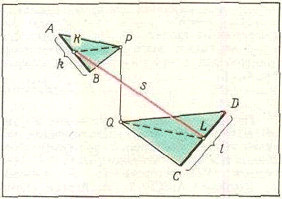
\includegraphics[width=8.5cm]{a}\\Рис. 6.
\abovedisplayskip = 0pt
\belowdisplayskip = 0pt
\abovedisplayshortskip = 0pt
\belowdisplayshortskip= 0pt
\

\

\

лежат отрезки $a$ и $b$. (В этой и следующих

формулах $a$, $пр_ab$ и т.п. означают длины со-

ответствующих отрезков.) Наименьший угол

между прямыми не превосходит $\pi/2$, поэто-

му $\cos\alpha\geqslant0$. Из (1) следует равенство
$$
a\:пр_ab=b\:пр_ba\eqno (2)
$$
которое пригодится нам для решения задачи.

\quad Обозначим через $P$ центр верхнего, а

через $Q$ - чентр нижнего оснований пирами-

ды. Мы докажем следующий факт, несколь-

ко более общий, чем нужное нам утвержде-

ние задачи \textbf{M168}.

\quad Пусть плоскости двух подобных равно-

бедренных треугольников $ABP$ и $CDQ$ с вер-

шинами $P$ и $Q$ перпендикулярны отрезку $PQ$

(и, тем самым, параллельны между собой).

Обозначим отрезок, соединяющий середины

$K$ и $L$ оснований $AB$ и $CD$, через $s$. Тогда

(Рис. 6.)
$$
пр_sk=пр_sl\eqno (3)
$$
Пользуясь (2), мы вместо (3) можем доказы-

вать такое равенство:
$$
k\:пр_ks=lпр_ls\eqno (4)
$$
Теперь воспользуемся тем, что как это сле-

дует из (1), длина пр $b_a$, не меняется при па-

раллельном переносе отрезков $a$ и $b$. Поэто-

му мы можем спроектировать отрезок $k = AB$

на плоскость треугольника $CDQ$ и получим:

$пр_{A' B'} K' L = пр_{A' B'} KL = пр_{A B} KL = $
\begin{flushright}
$=пр_ks$,\quad (5)
\end{flushright}
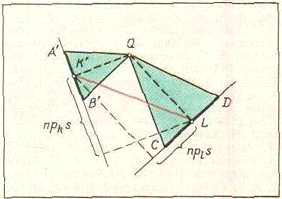
\includegraphics[width=8.5cm]{b}\\Рис. 7.
\end{minipage}
\hfill
\begin{minipage}[h]{0.45\linewidth}
где $A'$, $B'$ и $K'$ — проэкции точек $A$, $B$ и $K$

на плоскость $CDQ$ (рис. 7.). Таким образом,

мы свели задачу к тому случаю, когда оба

треугольника лежат в одной плоскости (и име-

ют общую вершину).

\quad Если отрезки $AB$ и $CD$ параллельны,

то равенсто (4) очевидно, поскольку обе

проэкции равны нулю.Если эти отрезки не-

параллельны, то получаем:

\Large $\frac{k}{l}=\frac{A' B'}{C D}=\frac{Q K'}{Q L}=\frac{\sin{\sphericalangle Q L K'}}{\sin{\sphericalangle {Q K' L}}}=$
\begin{flushright}
$=\frac{\mod{\cos{\sphericalangle K' L C}}}{\mod{\cos{\sphericalangle L K' B}}} = \frac{п р_l s}{п р_k s}$,
\end{flushright}

\normalsize откуда следует (4).

\

\

\

\quad \textbf{M169}. Пусть $k < n$ - натуральные чис-

ла. Расставьте числа 1, 2, 3, ..., $n^2$ в табли-

цу $n \times n$ так, чтобы в каждой строке чис-

ла шли в порядке возрастания и при этом

сумма чисел в $k$-м столбце была a) наимень-

шей; b) наибольшей.

\quad Решим сначала задачу a).

\quad Если расставить числа так, как показа-

но в таблице 1, $a$ --- сначала заполнить первые

$k$-столбцов, строку за строкой, числами от

1 до $kn$, а затем оставшимися числами запол-

нить последние $(n-k)$ столбцов (как угод-

но, лишь бы выполнялось условие возраста-

ния чисел в каждой строке)--- то сумма чи-

\

Т а б л и ц а \: 1a

\begin{center}
\begin{flushright}
$k$ \quad \quad \quad \quad \: \: \:
\end{flushright}
\begin{tabular}{ |c c c c|c|c| } 
 \hline
 1 & 2 & ... & $k-1$ & $k$ & $n k+1$ ... \\ 
$k+1$ & $k+2$ & ... & 2 $k-1$ & 2 $k$ &  \\ 
2 $k+1$ & 2 $k+2$ & ... & 3 $k-1$ & 3 $k$ &  \\ 
... & ... & ... & ... & & \\
$(n-k)k+1$ & & ... & $n k-1$ & $n k$ & . . . $n^2$ \\
&&&&&\\
 \hline
\end{tabular}
\end{center}

сел в $k$-м столбце будет равна
$$
k(1+2+...+n)=\frac{kn(n+1)}{2}. \eqno (1)
$$
Мы докажем, что это значение суммы явля-

ется наименьшим. Сначала докажем, что

если $a_1, a_2, ..., a_n$ --- числа $k$-го столбца, за-

нумерованные в порядке возрастания:
$$
a_1 < a_2 < ... < a_i < ... < a_n \eqno (2)
$$
то
$$
a_i \geqslant k_i. \eqno (3)
$$
Действительно, рассмотрим числа, стоящие

в тех же строках, где стоят $a_1, a_2, ..., a_i$,

и в первых $k$ столбцах. Из условия (2) и усло-

вия, что числа в строках стоят в возрастаю-

щем порядке, следует, что эти $k i$ чисел не пре-

восходят числа $a_i$. Следовательно, среди чи-

сел $1, 2, 3, ..., n^2$ имеется по крайней мере

$k i$ чисел, не превосходящих $a_i$. Отсюда вы-

текает (3). Сложив неравенства (3) по всем
\end{minipage}

\end{figure}

\end{document}

